\documentclass{beamer}
\usepackage[utf8]{inputenc}
\usepackage{ifpdf}
%\usepackage{hyperref}
\usepackage[english]{babel}
\usepackage{amsfonts}
\usepackage{amsmath}
\usepackage{amsthm}
\usepackage{stmaryrd}
\usepackage{color}
\usepackage{graphicx}
\usepackage{tikz}
\usepackage{suffix}
%\usepackage{multicol}
%\usepackage{moreverb}
\usepackage{listings}
%\usepackage{color}
%\usepackage{algorithm}
%\usepackage{algorithmicx}
%\usepackage{algpseudocode}
%\usepackage{longtable}
%\usepackage{geometry}
%\geometry{margin=2cm}
%\floatname{algorithm}{Algorithmus}
\usepackage{pgfpages}

% profiles and stuff
\newcommand{\profile}[1]{\left\llbracket #1 \right\rrbracket}
\newcommand{\profileconcat}{\circ}
%\newcommand{\profileones}[1]{\mathbb{1}^#1}
\newcommand{\profilerepeat}[2]{{(#1)}^{#2}}
\newcommand{\profileones}[1]{\profilerepeat{1}{#1}}

\newcommand{\E}[1]{\mathbb{E}\left[ #1 \right]}
\newcommand{\naturals}{\mathbb{N}}

\newcommand{\p}[1]{\operatorname{Pr}\left[#1\right]}
\newcommand{\alltasks}{{\mathbb T}}
\newcommand{\neededfor}{\rightarrow}
\WithSuffix\newcommand\neededfor*{\stackrel{*}{\rightarrow}}

\newenvironment{strategyblock}
{
  \begin{block}{Strategy}
}
{
  \end{block}
}

\newenvironment{motivationblock}
{
  \begin{block}{Motivation}
}
{
  \end{block}
}

\newenvironment{counterexampleblock}
{
  \begin{alertblock}{Counterexample}
}
{
  \end{alertblock}
}



\newcommand{\leveltop}{0}
\newcommand{\leveltopI}{0}
\newcommand{\leveltopII}{0}
\newcommand{\leveltopIII}{0}
\newcommand{\leveltopIIII}{0}
\newcommand{\leveltopIIIII}{0}
\newcommand{\leveltopIIIIII}{0}
\newcommand{\leveltopIIIIIII}{0}
\newcommand{\leveltopIIIIIIII}{0}
\newcommand{\leveltopIIIIIIIII}{0}
\newcommand{\leveltopIIIIIIIIII}{0}
\newcommand{\leveltopIIIIIIIIIII}{0}
\newcommand{\leveltopIIIIIIIIIIII}{0}
\newcommand{\leveltopIIIIIIIIIIIII}{0}
\newcommand{\leveltopIIIIIIIIIIIIII}{0}
\newcommand{\leveltopIIIIIIIIIIIIIII}{0}

\usetikzlibrary{decorations.pathmorphing}
\usetikzlibrary{decorations.pathreplacing}
\usetikzlibrary{shapes.callouts}
\usetikzlibrary{shapes.multipart,chains}
\usetikzlibrary{positioning}
\usetikzlibrary{matrix}
\usetikzlibrary{automata}
\usetikzlibrary{external} 
\tikzstyle{task_scheduled}=[fill=white, draw=black, task_cross]
\tikzstyle{task_cross}=[
    {path picture={ 
        \draw[black]
        (path picture bounding box.south east) -- 
        (path picture bounding box.north west) 
        (path picture bounding box.south west) -- 
        (path picture bounding box.north east);
      }
    }
]
\tikzset{onslide/.code args={<#1>#2}{%
  \only<#1>{\pgfkeysalso{#2}} 
}}

\title{Investigation of some Stochastic Scheduling Problems}
\subtitle{Master's Thesis in Computer Science}
\author[P. Müller]{Philipp Müller}
\institute[TUM]{Technische Universität München}
\date{November 20, 2013}

\usetheme[compress]{Singapore}
\useinnertheme{rectangles}

\DeclareMathOperator*{\argmax}{arg\,max}

\lstset{
	basicstyle=\ttfamily,
	tabsize=2
}

%\setbeameroption{show notes on second screen=left}

\setbeamertemplate{footline}
{
  \hbox{
    \begin{beamercolorbox}[wd=\paperwidth,ht=0.2cm,dp=0.2cm]{page footer}
      \begin{columns}
        \begin{column}{.33\paperwidth}
          \centering{}
        \end{column}
        \begin{column}{.33\paperwidth}
          \centering{}
          \insertframenumber 
        \end{column}
        \begin{column}{.33\paperwidth}
          \centering
        \end{column}
      \end{columns}
    \end{beamercolorbox}
  }
  \vskip0pt
}
\usenavigationsymbolstemplate{}

\newcommand{\todo}[1]{ {\color{red}{#1} }}

\tikzset{onslide/.code args={<#1>#2}{%
  \only<#1>{\pgfkeysalso{#2}} 
}}

%\usetheme[compress]{Berlin}

\AtBeginPart{
  \begin{frame}
    \partpage
    %\setcounter{tocdepth}{1}
    %\tableofcontents
  \end{frame}
}

\begin{document}

\begin{frame}
  \maketitle{}
\end{frame}

\section{Introduction}
\label{sec:intro}

\subsection{Problem statement}
\label{sec:problem-statement}

\begin{frame}
  \frametitle{Problem statement}
  \begin{itemize}
  \item Set of tasks
  \item Dependencies form intree structure
  \item Task times exponentially distributed with same parameter (w.l.o.g. $\lambda = 1$)
  \item Goal: Minimize total expected make span
  \end{itemize}
  \begin{center}
    \small
    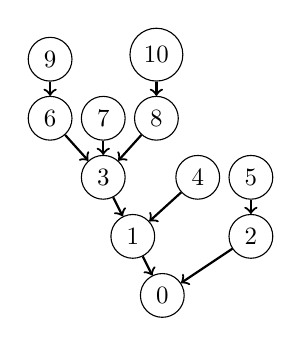
\begin{tikzpicture}[scale=.5, anchor=south]
      \node[circle, scale=0.9, draw] (tid0) at (3,1.5){0};
      \node[circle, scale=0.9, draw] (tid1) at (2.25,3){1};
      \node[circle, scale=0.9, draw] (tid2) at (1.5,4.5){3};
      \node[circle, scale=0.9, draw] (tid7) at (0.15,6){6};
      \node[circle, scale=0.9, draw] (tid9) at (0.15,7.5){9};
      \draw[<-, thick](tid7) -- (tid9);
      \node[circle, scale=0.9, draw] (tid10) at (1.5,6){7};
      \draw[<-, thick](tid2) -- (tid7);
      \draw[<-, thick](tid2) -- (tid10);
      \node[circle, scale=0.9, draw] (tid3) at (3.9,4.5){4};
      \node[circle, scale=0.9, draw] (tid5) at (2.85,6){8};
      \node[circle, scale=0.9, draw] (tid6) at (2.85,7.5){10
};
      \draw[<-, thick](tid5) -- (tid6);
      \draw[<-, thick](tid2) -- (tid5);
      \draw[<-, thick](tid1) -- (tid2);
      \draw[<-, thick](tid1) -- (tid3);
      \node[circle, scale=0.9, draw] (tid4) at (5.25,3){2};
      \node[circle, scale=0.9, draw] (tid8) at (5.25,4.5){5};
      \draw[<-, thick](tid4) -- (tid8);
      \draw[<-, thick](tid0) -- (tid1);
      \draw[<-, thick](tid0) -- (tid4);
    \end{tikzpicture}
  \end{center}
\end{frame}

\todo{Nonpreemtiv, etc (precise problem description!)}

\subsection{Schedules}
\label{sec:schedules}

\begin{frame}
  \frametitle{Schedules}
  \begin{itemize}
  \item A schedule describes the order in which tasks are processed
  \item Non-deterministic in our scenario (task times are random variables)
  \item Scheduling strategy influences expected make span
  \end{itemize}
\end{frame}

\begin{frame}
  \frametitle{Snapshots}
  \begin{itemize}
  \item Each state of a schedule is a snapshot
  \item Snapshot consists current intree and set of scheduled tasks
  \item A schedule can be visualized by a snapshot DAG
  \end{itemize}
\end{frame}

\begin{frame}
  \frametitle{Schedule visualization}
  \only<1>{
    \begin{center}
      \renewcommand{\leveltopI}{-15cm + \leveltop}
\renewcommand{\leveltopII}{-15cm + \leveltopI}
\renewcommand{\leveltopIII}{-16cm + \leveltopII}
\renewcommand{\leveltopIIII}{-12cm + \leveltopIII}
\renewcommand{\leveltopIIIII}{-12cm + \leveltopIIII}
\renewcommand{\leveltopIIIIII}{-12cm + \leveltopIIIII}
\renewcommand{\leveltopIIIIIII}{-12cm + \leveltopIIIIII}
\renewcommand{\leveltopIIIIIIII}{-12cm + \leveltopIIIIIII}
\renewcommand{\leveltopIIIIIIIII}{-12cm + \leveltopIIIIIIII}
\renewcommand{\leveltopIIIIIIIIII}{-12cm + \leveltopIIIIIIIII}
\renewcommand{\leveltopIIIIIIIIIII}{-12cm + \leveltopIIIIIIIIII}
\begin{tikzpicture}[scale=.13333, anchor=south]
  % legende
  \filldraw[dashed,fill=gray!10!white] (-20, -30) rectangle +(36.5, 12);
  % \draw[dashed] (-30, -13) -- +(60, 0);
  % \draw[dashed] (-30, -24) -- +(60, 0);
  % \node at (10, -21) {Intermediate snapshots};
  \begin{scope}[yshift=\leveltopI cm]
    \matrix (line1)[column sep=0.5cm, ampersand replacement=\&] {
      \node[draw=black, rectangle split,  rectangle split parts=1] (sn0x17d67b0){
        \begin{tikzpicture}[scale=.13333]
          \node[circle, scale=0.5, fill] (tid0) at (4.5,1.5){};
          \node[circle, scale=0.5, fill] (tid2) at (2.25,3){};
          \node[circle, scale=0.5, fill, task_scheduled] (tid4) at (2.25,4.5){};
          \draw[](tid2) -- (tid4);
          \node[circle, scale=0.5, fill] (tid3) at (6,3){};
          \node[circle, scale=0.5, fill] (tid5) at (3.75,4.5){};
          \node[circle, scale=0.5, fill] (tid6) at (5.25,4.5){};
          \node[circle, scale=0.5, fill] (tid7) at (7.5,4.5){};
          \node[circle, scale=0.5, fill] (tid8) at (6.75,6){};
          \node[circle, scale=0.5, fill] (tid9) at (8.25,6){};
          \node[circle, scale=0.5, fill, task_scheduled] (tid10) at (8.25,7.5){};
          \draw[](tid9) -- (tid10);
          \draw[](tid7) -- (tid8);
          \draw[](tid7) -- (tid9);
          \draw[](tid3) -- (tid5);
          \draw[](tid3) -- (tid6);
          \draw[](tid3) -- (tid7);
          \draw[](tid0) -- (tid2);
          \draw[](tid0) -- (tid3);
        \end{tikzpicture}
      }
      ;
      \& 
      \\
    };
  \end{scope}
  \begin{scope}[yshift=\leveltopII cm]
    \matrix (line2)[column sep=0.5cm, ampersand replacement=\&] {
      \node[draw=black, rectangle split,  rectangle split parts=1] (sn0x17d65a0){
        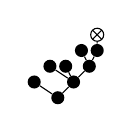
\begin{tikzpicture}[scale=.13333]
          \node[circle, scale=0.5, fill] (tid0) at (4.5,1.5){};
          \node[circle, scale=0.5, fill] (tid2) at (2.25,3){};
          \node[circle, scale=0.5, fill] (tid3) at (6,3){};
          \node[circle, scale=0.5, fill] (tid5) at (3.75,4.5){};
          \node[circle, scale=0.5, fill] (tid6) at (5.25,4.5){};
          \node[circle, scale=0.5, fill] (tid7) at (7.5,4.5){};
          \node[circle, scale=0.5, fill] (tid8) at (6.75,6){};
          \node[circle, scale=0.5, fill] (tid9) at (8.25,6){};
          \node[circle, scale=0.5, fill, task_scheduled] (tid10) at (8.25,7.5){};
          \draw[](tid9) -- (tid10);
          \draw[](tid7) -- (tid8);
          \draw[](tid7) -- (tid9);
          \draw[](tid3) -- (tid5);
          \draw[](tid3) -- (tid6);
          \draw[](tid3) -- (tid7);
          \draw[](tid0) -- (tid2);
          \draw[](tid0) -- (tid3);
        \end{tikzpicture}
      }
      ;
      \& 
      \node[minimum width=1cm]{};
      \&
      \node[draw=black, rectangle split,  rectangle split parts=1] (sn0x17d57c0){
        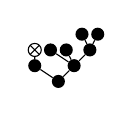
\begin{tikzpicture}[scale=.13333]
          \node[circle, scale=0.5, fill] (tid0) at (4.5,1.5){};
          \node[circle, scale=0.5, fill] (tid2) at (2.25,3){};
          \node[circle, scale=0.5, fill, task_scheduled] (tid4) at (2.25,4.5){};
          \draw[](tid2) -- (tid4);
          \node[circle, scale=0.5, fill] (tid3) at (6,3){};
          \node[circle, scale=0.5, fill] (tid5) at (3.75,4.5){};
          \node[circle, scale=0.5, fill] (tid6) at (5.25,4.5){};
          \node[circle, scale=0.5, fill] (tid7) at (7.5,4.5){};
          \node[circle, scale=0.5, fill] (tid8) at (6.75,6){};
          \node[circle, scale=0.5, fill] (tid9) at (8.25,6){};
          \draw[](tid7) -- (tid8);
          \draw[](tid7) -- (tid9);
          \draw[](tid3) -- (tid5);
          \draw[](tid3) -- (tid6);
          \draw[](tid3) -- (tid7);
          \draw[](tid0) -- (tid2);
          \draw[](tid0) -- (tid3);
        \end{tikzpicture}
      }
      ;
      \& 
      \\
    };
  \end{scope}
  \begin{scope}[yshift=\leveltopIII cm]
    \matrix (line3)[column sep=0.5cm, ampersand replacement=\&] {
      \node[draw=black, rectangle split,  rectangle split parts=1] (sn0x17d55b0){
        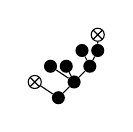
\begin{tikzpicture}[scale=.13333]
          \node[circle, scale=0.5, fill] (tid0) at (4.5,1.5){};
          \node[circle, scale=0.5, fill, task_scheduled] (tid2) at (2.25,3){};
          \node[circle, scale=0.5, fill] (tid3) at (6,3){};
          \node[circle, scale=0.5, fill] (tid5) at (3.75,4.5){};
          \node[circle, scale=0.5, fill] (tid6) at (5.25,4.5){};
          \node[circle, scale=0.5, fill] (tid7) at (7.5,4.5){};
          \node[circle, scale=0.5, fill] (tid8) at (6.75,6){};
          \node[circle, scale=0.5, fill] (tid9) at (8.25,6){};
          \node[circle, scale=0.5, fill, task_scheduled] (tid10) at (8.25,7.5){};
          \draw[](tid9) -- (tid10);
          \draw[](tid7) -- (tid8);
          \draw[](tid7) -- (tid9);
          \draw[](tid3) -- (tid5);
          \draw[](tid3) -- (tid6);
          \draw[](tid3) -- (tid7);
          \draw[](tid0) -- (tid2);
          \draw[](tid0) -- (tid3);
        \end{tikzpicture}
      }
      ;
      \& 
      \node[draw=black, rectangle split,  rectangle split parts=1] (sn0x17d6160){
        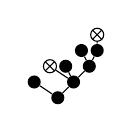
\begin{tikzpicture}[scale=.13333]
          \node[circle, scale=0.5, fill] (tid0) at (4.5,1.5){};
          \node[circle, scale=0.5, fill] (tid2) at (2.25,3){};
          \node[circle, scale=0.5, fill] (tid3) at (6,3){};
          \node[circle, scale=0.5, fill, task_scheduled] (tid5) at (3.75,4.5){};
          \node[circle, scale=0.5, fill] (tid6) at (5.25,4.5){};
          \node[circle, scale=0.5, fill] (tid7) at (7.5,4.5){};
          \node[circle, scale=0.5, fill] (tid8) at (6.75,6){};
          \node[circle, scale=0.5, fill] (tid9) at (8.25,6){};
          \node[circle, scale=0.5, fill, task_scheduled] (tid10) at (8.25,7.5){};
          \draw[](tid9) -- (tid10);
          \draw[](tid7) -- (tid8);
          \draw[](tid7) -- (tid9);
          \draw[](tid3) -- (tid5);
          \draw[](tid3) -- (tid6);
          \draw[](tid3) -- (tid7);
          \draw[](tid0) -- (tid2);
          \draw[](tid0) -- (tid3);
        \end{tikzpicture}
      }
      ;
      \& 
      \node[draw=black, rectangle split,  rectangle split parts=1] (sn0x17d5380){
        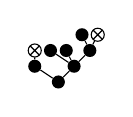
\begin{tikzpicture}[scale=.13333]
          \node[circle, scale=0.5, fill] (tid0) at (4.5,1.5){};
          \node[circle, scale=0.5, fill] (tid2) at (2.25,3){};
          \node[circle, scale=0.5, fill, task_scheduled] (tid4) at (2.25,4.5){};
          \draw[](tid2) -- (tid4);
          \node[circle, scale=0.5, fill] (tid3) at (6,3){};
          \node[circle, scale=0.5, fill] (tid5) at (3.75,4.5){};
          \node[circle, scale=0.5, fill] (tid6) at (5.25,4.5){};
          \node[circle, scale=0.5, fill] (tid7) at (7.5,4.5){};
          \node[circle, scale=0.5, fill] (tid8) at (6.75,6){};
          \node[circle, scale=0.5, fill, task_scheduled] (tid9) at (8.25,6){};
          \draw[](tid7) -- (tid8);
          \draw[](tid7) -- (tid9);
          \draw[](tid3) -- (tid5);
          \draw[](tid3) -- (tid6);
          \draw[](tid3) -- (tid7);
          \draw[](tid0) -- (tid2);
          \draw[](tid0) -- (tid3);
        \end{tikzpicture}
      }
      ;
      \& 
      \node[draw=black, rectangle split,  rectangle split parts=1] (sn0x17d2f50){
        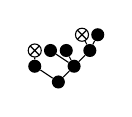
\begin{tikzpicture}[scale=.13333]
          \node[circle, scale=0.5, fill] (tid0) at (4.5,1.5){};
          \node[circle, scale=0.5, fill] (tid2) at (2.25,3){};
          \node[circle, scale=0.5, fill, task_scheduled] (tid4) at (2.25,4.5){};
          \draw[](tid2) -- (tid4);
          \node[circle, scale=0.5, fill] (tid3) at (6,3){};
          \node[circle, scale=0.5, fill] (tid5) at (3.75,4.5){};
          \node[circle, scale=0.5, fill] (tid6) at (5.25,4.5){};
          \node[circle, scale=0.5, fill] (tid7) at (7.5,4.5){};
          \node[circle, scale=0.5, fill, task_scheduled] (tid8) at (6.75,6){};
          \node[circle, scale=0.5, fill] (tid9) at (8.25,6){};
          \draw[](tid7) -- (tid8);
          \draw[](tid7) -- (tid9);
          \draw[](tid3) -- (tid5);
          \draw[](tid3) -- (tid6);
          \draw[](tid3) -- (tid7);
          \draw[](tid0) -- (tid2);
          \draw[](tid0) -- (tid3);
        \end{tikzpicture}
      }
      ;
      \& 
      \node[draw=black, rectangle split,  rectangle split parts=1] (sn0x17d3a00){
        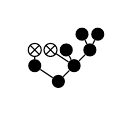
\begin{tikzpicture}[scale=.13333]
          \node[circle, scale=0.5, fill] (tid0) at (4.5,1.5){};
          \node[circle, scale=0.5, fill] (tid2) at (2.25,3){};
          \node[circle, scale=0.5, fill, task_scheduled] (tid4) at (2.25,4.5){};
          \draw[](tid2) -- (tid4);
          \node[circle, scale=0.5, fill] (tid3) at (6,3){};
          \node[circle, scale=0.5, fill, task_scheduled] (tid5) at (3.75,4.5){};
          \node[circle, scale=0.5, fill] (tid6) at (5.25,4.5){};
          \node[circle, scale=0.5, fill] (tid7) at (7.5,4.5){};
          \node[circle, scale=0.5, fill] (tid8) at (6.75,6){};
          \node[circle, scale=0.5, fill] (tid9) at (8.25,6){};
          \draw[](tid7) -- (tid8);
          \draw[](tid7) -- (tid9);
          \draw[](tid3) -- (tid5);
          \draw[](tid3) -- (tid6);
          \draw[](tid3) -- (tid7);
          \draw[](tid0) -- (tid2);
          \draw[](tid0) -- (tid3);
        \end{tikzpicture}
      }
      ;
      \& 
      \\
    };
  \end{scope}
  \draw (sn0x17d67b0.south) -- node[xshift=.4cm]{$0.5$} (sn0x17d57c0.north);
  \draw (sn0x17d67b0.south) -- node[left, yshift=.2cm]{$0.5$} (sn0x17d65a0.north);
  \draw (sn0x17d65a0.south) -- node[right]{$0.8$} (sn0x17d6160.north);
  \draw (sn0x17d65a0.south) -- node[left, xshift=-.25cm]{$0.2$} (sn0x17d55b0.north);
  \draw (sn0x17d57c0.south) -- node[right, xshift=.25]{$0.2$} (sn0x17d2f50.north);
  \draw (sn0x17d57c0.south) -- node[left, xshift=-3]{$0.4$} (sn0x17d5380.north);
  \draw (sn0x17d57c0.south) -- node[right, xshift=5]{$0.4$} (sn0x17d3a00.north);
\end{tikzpicture} % with intermediate snaps
    \end{center}
  }
  \only<2>{
    \begin{center}
      \input{talk_schedule_vis2} % without intermediate snaps
    \end{center}
  }
  \only<3>{
    \begin{center}
      \input{talk_schedule_vis3} % compressed form
    \end{center}
  }
\end{frame}

\begin{frame}
  \frametitle{Epected run time}
  \begin{itemize}
  \item $r$ tasks currently scheduled
  \item Compute run time recursively:
    \begin{itemize}
    \item Expected time for fastest task ($\frac{1}{r}$)
    \item Weighted expected time for successive snapshots
    \end{itemize}
  \end{itemize}
\end{frame}

\begin{frame}
  \only<1>{
    \begin{center}
      \input{talk_schedule_vis3} % compressed form
    \end{center}
  }
  \only<2>{
    \begin{center}
      \renewcommand{\leveltopI}{-25cm + \leveltop}
\renewcommand{\leveltopII}{-25cm + \leveltopI}
\renewcommand{\leveltopIII}{-16cm + \leveltopII}
\renewcommand{\leveltopIIII}{-12cm + \leveltopIII}
\renewcommand{\leveltopIIIII}{-12cm + \leveltopIIII}
\renewcommand{\leveltopIIIIII}{-12cm + \leveltopIIIII}
\renewcommand{\leveltopIIIIIII}{-12cm + \leveltopIIIIII}
\renewcommand{\leveltopIIIIIIII}{-12cm + \leveltopIIIIIII}
\renewcommand{\leveltopIIIIIIIII}{-12cm + \leveltopIIIIIIII}
\renewcommand{\leveltopIIIIIIIIII}{-12cm + \leveltopIIIIIIIII}
\renewcommand{\leveltopIIIIIIIIIII}{-12cm + \leveltopIIIIIIIIII}
\begin{tikzpicture}[scale=.13333, anchor=south]
  % legende
  %\filldraw[dashed,fill=gray!10!white] (-20, -30) rectangle +(36.5, 12);
  % \draw[dashed] (-30, -13) -- +(60, 0);
  % \draw[dashed] (-30, -24) -- +(60, 0);
  % \node at (10, -21) {Intermediate snapshots};
  \begin{scope}[yshift=\leveltopI cm]
    \matrix (line1)[column sep=0.5cm, ampersand replacement=\&] {
      \node[draw=black, rectangle split,  rectangle split parts=3] (sn0x17d67b0){
        \begin{tikzpicture}[scale=.13333]
          \node[circle, scale=0.5, fill] (tid0) at (4.5,1.5){};
          \node[circle, scale=0.5, fill] (tid2) at (2.25,3){};
          \node[circle, scale=0.5, fill, task_scheduled] (tid4) at (2.25,4.5){};
          \draw[](tid2) -- (tid4);
          \node[circle, scale=0.5, fill] (tid3) at (6,3){};
          \node[circle, scale=0.5, fill] (tid5) at (3.75,4.5){};
          \node[circle, scale=0.5, fill] (tid6) at (5.25,4.5){};
          \node[circle, scale=0.5, fill] (tid7) at (7.5,4.5){};
          \node[circle, scale=0.5, fill] (tid8) at (6.75,6){};
          \node[circle, scale=0.5, fill] (tid9) at (8.25,6){};
          \node[circle, scale=0.5, fill, task_scheduled] (tid10) at (8.25,7.5){};
          \draw[](tid9) -- (tid10);
          \draw[](tid7) -- (tid8);
          \draw[](tid7) -- (tid9);
          \draw[](tid3) -- (tid5);
          \draw[](tid3) -- (tid6);
          \draw[](tid3) -- (tid7);
          \draw[](tid0) -- (tid2);
          \draw[](tid0) -- (tid3);
        \end{tikzpicture}
        \nodepart{second}
        ? %6.43745
        \nodepart{third}
        \footnotesize{10\ 40\ 20\ 10\ 20}
      }
      ;
      \& 
      \\
    };
  \end{scope}
  \begin{scope}[yshift=\leveltopII cm]
    \matrix (line2)[column sep=.5cm, ampersand replacement=\&] {
      \node[draw=black, rectangle split,  rectangle split parts=2] (sn0x17d55b0){
        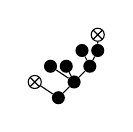
\begin{tikzpicture}[scale=.13333]
          \node[circle, scale=0.5, fill] (tid0) at (4.5,1.5){};
          \node[circle, scale=0.5, fill, task_scheduled] (tid2) at (2.25,3){};
          \node[circle, scale=0.5, fill] (tid3) at (6,3){};
          \node[circle, scale=0.5, fill] (tid5) at (3.75,4.5){};
          \node[circle, scale=0.5, fill] (tid6) at (5.25,4.5){};
          \node[circle, scale=0.5, fill] (tid7) at (7.5,4.5){};
          \node[circle, scale=0.5, fill] (tid8) at (6.75,6){};
          \node[circle, scale=0.5, fill] (tid9) at (8.25,6){};
          \node[circle, scale=0.5, fill, task_scheduled] (tid10) at (8.25,7.5){};
          \draw[](tid9) -- (tid10);
          \draw[](tid7) -- (tid8);
          \draw[](tid7) -- (tid9);
          \draw[](tid3) -- (tid5);
          \draw[](tid3) -- (tid6);
          \draw[](tid3) -- (tid7);
          \draw[](tid0) -- (tid2);
          \draw[](tid0) -- (tid3);
        \end{tikzpicture}
        \nodepart{second}
        6.1640
      }
      ;
      \& 
      \node[draw=black, rectangle split,  rectangle split parts=2] (sn0x17d6160){
        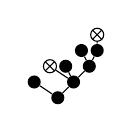
\begin{tikzpicture}[scale=.13333]
          \node[circle, scale=0.5, fill] (tid0) at (4.5,1.5){};
          \node[circle, scale=0.5, fill] (tid2) at (2.25,3){};
          \node[circle, scale=0.5, fill] (tid3) at (6,3){};
          \node[circle, scale=0.5, fill, task_scheduled] (tid5) at (3.75,4.5){};
          \node[circle, scale=0.5, fill] (tid6) at (5.25,4.5){};
          \node[circle, scale=0.5, fill] (tid7) at (7.5,4.5){};
          \node[circle, scale=0.5, fill] (tid8) at (6.75,6){};
          \node[circle, scale=0.5, fill] (tid9) at (8.25,6){};
          \node[circle, scale=0.5, fill, task_scheduled] (tid10) at (8.25,7.5){};
          \draw[](tid9) -- (tid10);
          \draw[](tid7) -- (tid8);
          \draw[](tid7) -- (tid9);
          \draw[](tid3) -- (tid5);
          \draw[](tid3) -- (tid6);
          \draw[](tid3) -- (tid7);
          \draw[](tid0) -- (tid2);
          \draw[](tid0) -- (tid3);
        \end{tikzpicture}
        \nodepart{second}
        5.9921
      }
      ;
      \& 
      \node[draw=black, rectangle split,  rectangle split parts=2] (sn0x17d5380){
        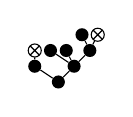
\begin{tikzpicture}[scale=.13333]
          \node[circle, scale=0.5, fill] (tid0) at (4.5,1.5){};
          \node[circle, scale=0.5, fill] (tid2) at (2.25,3){};
          \node[circle, scale=0.5, fill, task_scheduled] (tid4) at (2.25,4.5){};
          \draw[](tid2) -- (tid4);
          \node[circle, scale=0.5, fill] (tid3) at (6,3){};
          \node[circle, scale=0.5, fill] (tid5) at (3.75,4.5){};
          \node[circle, scale=0.5, fill] (tid6) at (5.25,4.5){};
          \node[circle, scale=0.5, fill] (tid7) at (7.5,4.5){};
          \node[circle, scale=0.5, fill] (tid8) at (6.75,6){};
          \node[circle, scale=0.5, fill, task_scheduled] (tid9) at (8.25,6){};
          \draw[](tid7) -- (tid8);
          \draw[](tid7) -- (tid9);
          \draw[](tid3) -- (tid5);
          \draw[](tid3) -- (tid6);
          \draw[](tid3) -- (tid7);
          \draw[](tid0) -- (tid2);
          \draw[](tid0) -- (tid3);
        \end{tikzpicture}
        \nodepart{second}
        5.8203
      }
      ;
      \& 
      \node[draw=black, rectangle split,  rectangle split parts=2] (sn0x17d2f50){
        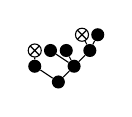
\begin{tikzpicture}[scale=.13333]
          \node[circle, scale=0.5, fill] (tid0) at (4.5,1.5){};
          \node[circle, scale=0.5, fill] (tid2) at (2.25,3){};
          \node[circle, scale=0.5, fill, task_scheduled] (tid4) at (2.25,4.5){};
          \draw[](tid2) -- (tid4);
          \node[circle, scale=0.5, fill] (tid3) at (6,3){};
          \node[circle, scale=0.5, fill] (tid5) at (3.75,4.5){};
          \node[circle, scale=0.5, fill] (tid6) at (5.25,4.5){};
          \node[circle, scale=0.5, fill] (tid7) at (7.5,4.5){};
          \node[circle, scale=0.5, fill, task_scheduled] (tid8) at (6.75,6){};
          \node[circle, scale=0.5, fill] (tid9) at (8.25,6){};
          \draw[](tid7) -- (tid8);
          \draw[](tid7) -- (tid9);
          \draw[](tid3) -- (tid5);
          \draw[](tid3) -- (tid6);
          \draw[](tid3) -- (tid7);
          \draw[](tid0) -- (tid2);
          \draw[](tid0) -- (tid3);
        \end{tikzpicture}
        \nodepart{second}
        5.8203
      }
      ;
      \& 
      \node[draw=black, rectangle split,  rectangle split parts=2] (sn0x17d3a00){
        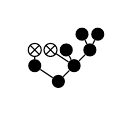
\begin{tikzpicture}[scale=.13333]
          \node[circle, scale=0.5, fill] (tid0) at (4.5,1.5){};
          \node[circle, scale=0.5, fill] (tid2) at (2.25,3){};
          \node[circle, scale=0.5, fill, task_scheduled] (tid4) at (2.25,4.5){};
          \draw[](tid2) -- (tid4);
          \node[circle, scale=0.5, fill] (tid3) at (6,3){};
          \node[circle, scale=0.5, fill, task_scheduled] (tid5) at (3.75,4.5){};
          \node[circle, scale=0.5, fill] (tid6) at (5.25,4.5){};
          \node[circle, scale=0.5, fill] (tid7) at (7.5,4.5){};
          \node[circle, scale=0.5, fill] (tid8) at (6.75,6){};
          \node[circle, scale=0.5, fill] (tid9) at (8.25,6){};
          \draw[](tid7) -- (tid8);
          \draw[](tid7) -- (tid9);
          \draw[](tid3) -- (tid5);
          \draw[](tid3) -- (tid6);
          \draw[](tid3) -- (tid7);
          \draw[](tid0) -- (tid2);
          \draw[](tid0) -- (tid3);
        \end{tikzpicture}
        \nodepart{second}
        5.8906
      }
      ;
      \& 
      \\
    };
  \end{scope}
  \draw (sn0x17d67b0.south) -- (sn0x17d6160.north);
  \draw (sn0x17d67b0.south) -- (sn0x17d55b0.north);
  \draw (sn0x17d67b0.south) -- (sn0x17d2f50.north);
  \draw (sn0x17d67b0.south) -- (sn0x17d5380.north);
  \draw (sn0x17d67b0.south) -- (sn0x17d3a00.north);
  \draw[decorate, decoration=brace] (sn0x17d3a00.north) ++ (0,14) --node [right]{Exp. $\frac{1}{2}$} ++ (0,-13); 
\end{tikzpicture} % expected run times
    \end{center}
  }
  \begin{equation*}
    \frac{1}{2}
    + 0.1 \cdot 6.1640
    + 0.4 \cdot 5.9921
    + 0.2 \cdot 5.8203
    + \dots
    % + 0.1 \cdot 5.8203
    % + 0.2 \cdot 5.8906
    = 6.43745
  \end{equation*}
\end{frame}

\begin{frame}
  \frametitle{Equivalent snapshots}
  \begin{itemize}
  \item The following two snapshots (basically) describe the same problem:
    \todo{Bilder!}
  \item Isomorphic intrees
  \item Scheduled tasks are mapped onto each other
  \item Isomorphic snapshots can be excluded/re-used if they result from the same finishing task
  \end{itemize}
\end{frame}

\begin{frame}
  \frametitle{Equivalent snapshots --- example}
  \begin{center}
    \only<1>{
      \input{talk_equivalence_large}
    }
    \only<2>{
      \renewcommand{\leveltopI}{-10cm + \leveltop}
\renewcommand{\leveltopII}{-10cm + \leveltopI}
\begin{tikzpicture}[scale=.2, anchor=south]
  \begin{scope}[yshift=\leveltopI cm]
    \matrix (line1)[column sep=0.25cm] {
      \node[draw=black, rectangle split,  rectangle split parts=1] (sn0x9bc9928){
        \begin{tikzpicture}[scale=.2]
          \node[circle, scale=0.75, fill, draw=black] (tid0) at (3.75,1.5){};
          \node[circle, scale=0.75, fill, draw=black] (tid1) at (1.5,3){};
          \node[circle, scale=0.75, fill, task_scheduled] (tid4) at (0.75,4.5){};
          \node[circle, scale=0.75, fill, task_scheduled] (tid6) at (2.25,4.5){};
          \draw[](tid1) -- (tid4);
          \draw[](tid1) -- (tid6);
          \node[circle, scale=0.75, fill, task_scheduled] (tid2) at (3.75,3){};
          \node[circle, scale=0.75, fill, draw=black] (tid3) at (5.25,3){};
          \node[circle, scale=0.75, fill, draw=black] (tid5) at (6.75,3){};
          \draw[](tid0) -- (tid1);
          \draw[](tid0) -- (tid2);
          \draw[](tid0) -- (tid3);
          \draw[](tid0) -- (tid5);
        \end{tikzpicture}
      };
      & 
      \\
    };
  \end{scope}
  \begin{scope}[yshift=\leveltopII cm]
    \matrix (line2)[column sep=0.25cm] {
      \node[draw=black, rectangle split,  rectangle split parts=1] (sn0x9bd2140){
        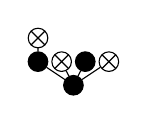
\begin{tikzpicture}[scale=.2]
          \node[circle, scale=0.75, fill, draw=black] (tid0) at (3,1.5){};
          \node[circle, scale=0.75, fill, draw=black] (tid1) at (0.75,3){};
          \node[circle, scale=0.75, fill, task_scheduled] (tid4) at (0.75,4.5){};
          \draw[](tid1) -- (tid4);
          \node[circle, scale=0.75, fill, task_scheduled] (tid2) at (2.25,3){};
          \node[circle, scale=0.75, fill, draw=black] (tid3) at (3.75,3){};
          \node[circle, scale=0.75, fill, task_scheduled] (tid5) at (5.25,3){};
          \draw[](tid0) -- (tid1);
          \draw[](tid0) -- (tid2);
          \draw[](tid0) -- (tid3);
          \draw[](tid0) -- (tid5);
        \end{tikzpicture}
      };
      & 
      \node[draw=black, rectangle split,  rectangle split parts=1] (sn0x9bc7440){
        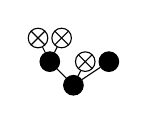
\begin{tikzpicture}[scale=.2]
          \node[circle, scale=0.75, fill, draw=black] (tid0) at (3,1.5){};
          \node[circle, scale=0.75, fill, draw=black] (tid1) at (1.5,3){};
          \node[circle, scale=0.75, fill, task_scheduled] (tid4) at (0.75,4.5){};
          \node[circle, scale=0.75, fill, task_scheduled] (tid6) at (2.25,4.5){};
          \draw[](tid1) -- (tid4);
          \draw[](tid1) -- (tid6);
          \node[circle, scale=0.75, fill, task_scheduled] (tid3) at (3.75,3){};
          \node[circle, scale=0.75, fill, draw=black] (tid5) at (5.25,3){};
          \draw[](tid0) -- (tid1);
          \draw[](tid0) -- (tid3);
          \draw[](tid0) -- (tid5);
        \end{tikzpicture}
      };
      & 
      \\
    };
  \end{scope}
  \draw[] (sn0x9bc9928.south) --node[right,xshift=.1cm]{$\frac{2}{6}$} (sn0x9bc7440.north);
  \draw[] (sn0x9bc9928.south) --node[left,xshift=-.1cm]{$\frac{4}{6}$} (sn0x9bd2140.north);
\end{tikzpicture}

    }
  \end{center}
\end{frame}

\section{Two processors}

\subsection{Optimal solution}

\begin{frame}
  \frametitle{Optimal solution}
  \begin{itemize}
  \item Highest-level-first (HLF) is optimal for two processors
  \item Profile (number of tasks per level) completely determines run time
  \end{itemize}
  \begin{exampleblock}{Profiles: Intrees with profile $\profile{6,3,1}$:}
    \begin{center}
      \includegraphics{../thesis/p2/four_profiles_631.pdf}  
    \end{center}
  \end{exampleblock}
\end{frame}

\subsection{Expected run time}

\begin{frame}
  \frametitle{Expected run time}
  \begin{block}{Function $SUC$:}
    \begin{equation*}
      SUC(\profile{n_1,\dots,n_r}) = \profile{n_1, n_2, n_3,\dots,n_{j-1},n_j-1,n_{j+1},\dots,n_r} 
    \end{equation*}
    such that $j$ is the minimum index such that $n_j>1$.  
  \end{block}
  \begin{block}{Optimal (i.e. HLF) expected run time}
    Let $P=\profile{n_1}\profileconcat P'$. Then
    \begin{equation*}
      \E{P} =
      \begin{cases}
        r, & \text{ if } P = \profile{\profileones r} \\
        \frac{1}{2} + \E{\profile{n_1-1}\profileconcat P'} , & \text{ if } n_1\geq 2 \\
        \frac{1}{2} + \frac{1}{2} \cdot \left( \E{P'} + \E{SUC(P)} \right) ,& \text{ otherwise } 
      \end{cases}.
    \end{equation*}
  \end{block}
\end{frame}

\begin{frame}
  \frametitle{Expected run time --- two-leaves intrees}
  \begin{theorem}[Moritz Maaß\todo{Wie zitieren?}]
    Let $l, k\in\naturals$, $a\in\naturals_0$. Intrees with profile $\profile{\profilerepeat{1}{l-k}, \profilerepeat{2}{k}, \profilerepeat{1}{a+1}}$ have expected run time
    \begin{align*}
      & \sum_{i=1}^k \left(\frac{1}{2}\right)^{l+i-1} \cdot \binom{l+i-2}{i-1} \cdot \left( k-i+2 \right) \\
       & + \sum_{j=1}^l \left(\frac{1}{2}\right)^{k+j-1} \cdot \binom{k+j-2}{j-1} \cdot \left( l-j+2 \right) \\
       & + \sum_{i=1}^k \sum_{j=1}^l \left( \frac{1}{2}^{k-i+l-j+1}\cdot\binom{ki+l-j}{l-j} \right) \\
       & + a
      .
    \end{align*}
  \end{theorem}
\end{frame}

\begin{frame}
  \frametitle{Expected run time --- intrees with many 1-levels}
  \begin{theorem}
    Intrees with profile $\profile{n_1,\profileones{j-2},n_j,\profileones{r-j}}$ (for $j\geq 2$) has expected run time
    \begin{equation*}
      \E{\profile{n_1,\profileones{j-2},n_j,\profileones{r-j}}} = 
      r + \frac{A_0(n_1-2)}{2^{n_1-1}} + \frac{A_{j-1}(n_j-2)}{2^{n_j+j-2}},
    \end{equation*}
    where $A_i$ is inductively defined as follows:
    \begin{equation*}
      A_0(n) = (n+1) \cdot 2^n \quad 
      A_{i+1}(n) = \sum_{k=0}^n A_{i}(k)
    \end{equation*}
  \end{theorem}
\end{frame}

\subsection{Profile DAG}

\begin{frame}
  \frametitle{Profile DAG}
  \begin{itemize}
  \item We can use profiles instead of whole snapshots
  \item Scheduled tasks are given implicitly
  \item Worst case profile $\profile{ \profileones{ \left\lfloor\frac{n}{2} \right\rfloor - 1}, \left\lceil \frac{n}{2} \right\rceil, 1 }$
  \item Worst case profile DAG size has $\lfloor \frac{n}{2} \rfloor \cdot \lceil \frac{n}{2} \rceil +1$ ``profile snapshots''.
  \item Each profile snapshot accounts for at most $\binom{n}{2}\in O(n^2)$ ``original snapshots''.
    
    $\Rightarrow$ Simple proof: At most $O(n^4)$ original snapshots.
  \end{itemize}
\end{frame}

\section{Program}

\begin{frame}
  \frametitle{Practical results}
  \begin{itemize}
  \item Excluding equivalent snapshots speeds up the program by at least factor 3 (for intrees with 11 or more tasks)
  \item Computing optimal schedules for all intrees with up to 15 tasks in 11 minutes and less than 2Gb of main memory
  \item More tasks require too much memory
  \item Computing optimal schedules for non-trivial intrees with 19 tasks takes one day
  \item Using Boost Rational to represent expectancies as fractions requires slightly more time and memory
  \item Using GMP to represent expectancies as fractions requires roughly doubles time and increases memory consumption by roughly 40\%
  \end{itemize}
\end{frame}

\section{Suboptimal strategies}

\subsection{HLF}

\begin{frame}
  \frametitle{Highest level first --- ambiguities}
  \begin{columns}
  \begin{column}{.5\textwidth}
    \centering
    \renewcommand{\leveltopI}{-12cm + \leveltop}
    \renewcommand{\leveltopII}{-12cm + \leveltopI}
    \renewcommand{\leveltopIII}{-12cm + \leveltopII}
    \renewcommand{\leveltopIIII}{-15cm + \leveltopIII}
    \renewcommand{\leveltopIIIII}{-15cm + \leveltopIIII}
    \renewcommand{\leveltopIIIIII}{-15cm + \leveltopIIIII}
    \renewcommand{\leveltopIIIIIII}{-15cm + \leveltopIIIIII}
    \begin{tikzpicture}[scale=.2, anchor=south]
      \begin{scope}[yshift=\leveltopI cm]
        \matrix (line1)[column sep=1cm] {
          \node[draw=black, rectangle split,  rectangle split parts=3] (sn0x938eff0){
            \begin{tikzpicture}[scale=.2]
              \node[circle, scale=0.75, fill] (tid0) at (3,1.5){};
              \node[circle, scale=0.75, fill] (tid1) at (2.25,3){};
              \node[circle, scale=0.75, fill, task_scheduled] (tid3) at (0.75,4.5){};
              \node[circle, scale=0.75, fill, task_scheduled] (tid4) at (2.25,4.5){};
              \node[circle, scale=0.75, fill, task_scheduled] (tid5) at (3.75,4.5){};
              \draw[](tid1) -- (tid3);
              \draw[](tid1) -- (tid4);
              \draw[](tid1) -- (tid5);
              \node[circle, scale=0.75, fill] (tid2) at (5.25,3){};
              \node[circle, scale=0.75, fill] (tid6) at (5.25,4.5){};
              \draw[](tid2) -- (tid6);
              \draw[](tid0) -- (tid1);
              \draw[](tid0) -- (tid2);
            \end{tikzpicture}
            \nodepart{two}
            \footnotesize{4.38889}
            \nodepart{three}
            \footnotesize{$100$}
          };
          \\
        };
      \end{scope}
      \begin{scope}[yshift=\leveltopII cm]
        \matrix (line2)[column sep=1cm] {
          \node[draw=black, rectangle split,  rectangle split parts=3] (sn0x938dbf0){
            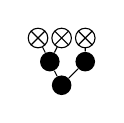
\begin{tikzpicture}[scale=.2]
              \node[circle, scale=0.75, fill] (tid0) at (2.25,1.5){};
              \node[circle, scale=0.75, fill] (tid1) at (1.5,3){};
              \node[circle, scale=0.75, fill, task_scheduled] (tid3) at (0.75,4.5){};
              \node[circle, scale=0.75, fill, task_scheduled] (tid4) at (2.25,4.5){};
              \draw[](tid1) -- (tid3);
              \draw[](tid1) -- (tid4);
              \node[circle, scale=0.75, fill] (tid2) at (3.75,3){};
              \node[circle, scale=0.75, fill, task_scheduled] (tid5) at (3.75,4.5){};
              \draw[](tid2) -- (tid5);
              \draw[](tid0) -- (tid1);
              \draw[](tid0) -- (tid2);
            \end{tikzpicture}
            \nodepart{two}
            \footnotesize{4.05556}
            \nodepart{three}
            \footnotesize{$33\:67$}
          };
          \\
        };
      \end{scope}
      \draw (sn0x938eff0.south) -- (sn0x938dbf0.north);
    \end{tikzpicture}    
  \end{column}
  \begin{column}{.5\textwidth}
    \centering
    \renewcommand{\leveltopI}{-12cm + \leveltop}
    \renewcommand{\leveltopII}{-12cm + \leveltopI}
    \renewcommand{\leveltopIII}{-12cm + \leveltopII}
    \renewcommand{\leveltopIIII}{-15cm + \leveltopIII}
    \renewcommand{\leveltopIIIII}{-15cm + \leveltopIIII}
    \renewcommand{\leveltopIIIIII}{-15cm + \leveltopIIIII}
    \renewcommand{\leveltopIIIIIII}{-15cm + \leveltopIIIIII}
    \begin{tikzpicture}[scale=.2, anchor=south]
      \begin{scope}[yshift=\leveltopI cm]
        \matrix (line1)[column sep=1cm] {
          \node[draw=black, rectangle split,  rectangle split parts=3] (sn0x938dc98){
            \begin{tikzpicture}[scale=.2]
              \node[circle, scale=0.75, fill] (tid0) at (3,1.5){};
              \node[circle, scale=0.75, fill] (tid1) at (2.25,3){};
              \node[circle, scale=0.75, fill, task_scheduled] (tid3) at (0.75,4.5){};
              \node[circle, scale=0.75, fill, task_scheduled] (tid4) at (2.25,4.5){};
              \node[circle, scale=0.75, fill] (tid5) at (3.75,4.5){};
              \draw[](tid1) -- (tid3);
              \draw[](tid1) -- (tid4);
              \draw[](tid1) -- (tid5);
              \node[circle, scale=0.75, fill] (tid2) at (5.25,3){};
              \node[circle, scale=0.75, fill, task_scheduled] (tid6) at (5.25,4.5){};
              \draw[](tid2) -- (tid6);
              \draw[](tid0) -- (tid1);
              \draw[](tid0) -- (tid2);
            \end{tikzpicture}
            \nodepart{two}
            \footnotesize{4.37037}
            \nodepart{three}
            \footnotesize{$33\:67$}
          };
          \\
        };
      \end{scope}
      \begin{scope}[yshift=\leveltopII cm]
        \matrix (line2)[column sep=1cm] {
          \node[draw=black, rectangle split,  rectangle split parts=3] (sn0x938d9b8){
            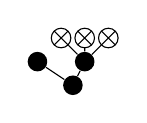
\begin{tikzpicture}[scale=.2]
              \node[circle, scale=0.75, fill] (tid0) at (3,1.5){};
              \node[circle, scale=0.75, fill] (tid1) at (0.75,3){};
              \node[circle, scale=0.75, fill] (tid2) at (3.75,3){};
              \node[circle, scale=0.75, fill, task_scheduled] (tid3) at (2.25,4.5){};
              \node[circle, scale=0.75, fill, task_scheduled] (tid4) at (3.75,4.5){};
              \node[circle, scale=0.75, fill, task_scheduled] (tid5) at (5.25,4.5){};
              \draw[](tid2) -- (tid3);
              \draw[](tid2) -- (tid4);
              \draw[](tid2) -- (tid5);
              \draw[](tid0) -- (tid1);
              \draw[](tid0) -- (tid2);
            \end{tikzpicture}
            \nodepart{two}
            \footnotesize{4}
            \nodepart{three}
            \footnotesize{$100$}
          };
          & 
          \node[draw=black, rectangle split,  rectangle split parts=3] (sn0x938dbf0){
            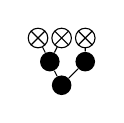
\begin{tikzpicture}[scale=.2]
              \node[circle, scale=0.75, fill] (tid0) at (2.25,1.5){};
              \node[circle, scale=0.75, fill] (tid1) at (1.5,3){};
              \node[circle, scale=0.75, fill, task_scheduled] (tid3) at (0.75,4.5){};
              \node[circle, scale=0.75, fill, task_scheduled] (tid4) at (2.25,4.5){};
              \draw[](tid1) -- (tid3);
              \draw[](tid1) -- (tid4);
              \node[circle, scale=0.75, fill] (tid2) at (3.75,3){};
              \node[circle, scale=0.75, fill, task_scheduled] (tid5) at (3.75,4.5){};
              \draw[](tid2) -- (tid5);
              \draw[](tid0) -- (tid1);
              \draw[](tid0) -- (tid2);
            \end{tikzpicture}
            \nodepart{two}
            \footnotesize{4.05556}
            \nodepart{three}
            \footnotesize{$33\:67$}
          };
          \\
        };
      \end{scope}
      \draw (sn0x938dc98.south) -- (sn0x938dbf0.north);
      \draw (sn0x938dc98.south) -- (sn0x938d9b8.north);
    \end{tikzpicture}
  \end{column}
\end{columns}
%%% Local Variables:
%%% TeX-master: "talk.tex"
%%% End: 

\end{frame}

\begin{frame}
  \frametitle{Highest level first --- strictly suboptimal}
  \begin{columns}[ht]
    \begin{column}{.45\textwidth}
      \centering
      \renewcommand{\leveltopI}{-16cm + \leveltop}
\renewcommand{\leveltopII}{-16cm + \leveltopI}
\renewcommand{\leveltopIII}{-16cm + \leveltopII}
\renewcommand{\leveltopIIII}{-16cm + \leveltopIII}
\renewcommand{\leveltopIIIII}{-16cm + \leveltopIIII}
\renewcommand{\leveltopIIIIII}{-16cm + \leveltopIIIII}
\renewcommand{\leveltopIIIIIII}{-16cm + \leveltopIIIIII}
\renewcommand{\leveltopIIIIIIII}{-16cm + \leveltopIIIIIII}
\renewcommand{\leveltopIIIIIIIII}{-16cm + \leveltopIIIIIIII}
\renewcommand{\leveltopIIIIIIIIII}{-16cm + \leveltopIIIIIIIII}
\renewcommand{\leveltopIIIIIIIIIII}{-16cm + \leveltopIIIIIIIIII}
\begin{tikzpicture}[scale=.2, anchor=south]
\begin{scope}[yshift=\leveltopI cm]
\matrix (line1)[column sep=0.5cm] {
\node[draw=black, rectangle split,  rectangle split parts=3] (sn0x9d41c38){
\begin{tikzpicture}[scale=.2]
\node[circle, scale=0.75, fill] (tid0) at (3,1.5){};
\node[circle, scale=0.75, fill] (tid1) at (0.75,3){};
\node[circle, scale=0.75, fill] (tid3) at (0.75,4.5){};
\node[circle, scale=0.75, fill] (tid5) at (0.75,6){};
\draw[](tid3) -- (tid5);
\draw[](tid1) -- (tid3);
\node[circle, scale=0.75, fill] (tid2) at (3.75,3){};
\node[circle, scale=0.75, fill] (tid4) at (3.75,4.5){};
\node[circle, scale=0.75, fill] (tid6) at (3.75,6){};
\node[circle, scale=0.75, fill, task_scheduled] (tid7) at (2.25,7.5){};
\node[circle, scale=0.75, fill] (tid8) at (4.5,7.5){};
\node[circle, scale=0.75, fill, task_scheduled] (tid9) at (3.75,9){};
\node[circle, scale=0.75, fill, task_scheduled] (tid10) at (5.25,9){};
\draw[](tid8) -- (tid9);
\draw[](tid8) -- (tid10);
\draw[](tid6) -- (tid7);
\draw[](tid6) -- (tid8);
\draw[](tid4) -- (tid6);
\draw[](tid2) -- (tid4);
\draw[](tid0) -- (tid1);
\draw[](tid0) -- (tid2);
\end{tikzpicture}
\nodepart{two}
\footnotesize{6.96798}
\nodepart{three}
\footnotesize{$67\:33$}
};
\\
};
\end{scope}
\begin{scope}[yshift=\leveltopII cm]
\matrix (line2)[column sep=0.5cm] {
\node[draw=black, rectangle split,  rectangle split parts=3] (sn0x9d41970){
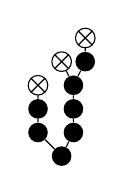
\begin{tikzpicture}[scale=.2]
\node[circle, scale=0.75, fill] (tid0) at (2.25,1.5){};
\node[circle, scale=0.75, fill] (tid1) at (0.75,3){};
\node[circle, scale=0.75, fill] (tid3) at (0.75,4.5){};
\node[circle, scale=0.75, fill, task_scheduled] (tid5) at (0.75,6){};
\draw[](tid3) -- (tid5);
\draw[](tid1) -- (tid3);
\node[circle, scale=0.75, fill] (tid2) at (3,3){};
\node[circle, scale=0.75, fill] (tid4) at (3,4.5){};
\node[circle, scale=0.75, fill] (tid6) at (3,6){};
\node[circle, scale=0.75, fill, task_scheduled] (tid7) at (2.25,7.5){};
\node[circle, scale=0.75, fill] (tid8) at (3.75,7.5){};
\node[circle, scale=0.75, fill, task_scheduled] (tid9) at (3.75,9){};
\draw[](tid8) -- (tid9);
\draw[](tid6) -- (tid7);
\draw[](tid6) -- (tid8);
\draw[](tid4) -- (tid6);
\draw[](tid2) -- (tid4);
\draw[](tid0) -- (tid1);
\draw[](tid0) -- (tid2);
\end{tikzpicture}
\nodepart{two}
\footnotesize{6.56279}
\nodepart{three}
\footnotesize{$33\:33\:33$}
};
 & 
\node[draw=black, rectangle split,  rectangle split parts=3] (sn0x9d41468){
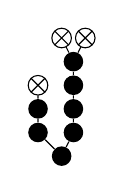
\begin{tikzpicture}[scale=.2]
\node[circle, scale=0.75, fill] (tid0) at (2.25,1.5){};
\node[circle, scale=0.75, fill] (tid1) at (0.75,3){};
\node[circle, scale=0.75, fill] (tid3) at (0.75,4.5){};
\node[circle, scale=0.75, fill, task_scheduled] (tid5) at (0.75,6){};
\draw[](tid3) -- (tid5);
\draw[](tid1) -- (tid3);
\node[circle, scale=0.75, fill] (tid2) at (3,3){};
\node[circle, scale=0.75, fill] (tid4) at (3,4.5){};
\node[circle, scale=0.75, fill] (tid6) at (3,6){};
\node[circle, scale=0.75, fill] (tid7) at (3,7.5){};
\node[circle, scale=0.75, fill, task_scheduled] (tid8) at (2.25,9){};
\node[circle, scale=0.75, fill, task_scheduled] (tid9) at (3.75,9){};
\draw[](tid7) -- (tid8);
\draw[](tid7) -- (tid9);
\draw[](tid6) -- (tid7);
\draw[](tid4) -- (tid6);
\draw[](tid2) -- (tid4);
\draw[](tid0) -- (tid1);
\draw[](tid0) -- (tid2);
\end{tikzpicture}
\nodepart{two}
\footnotesize{6.77836}
\nodepart{three}
\footnotesize{$67\:33$}
};
\\
};
\end{scope}
\draw (sn0x9d41c38.south) -- (sn0x9d41468.north);
\draw (sn0x9d41c38.south) -- (sn0x9d41970.north);
\end{tikzpicture}
%%% Local Variables:
%%% TeX-master: "thesis/thesis.tex"
%%% End: 

    \end{column}
    \begin{column}{.45\textwidth}
      \centering
      \input{0012346688_opt}
    \end{column}
  \end{columns}
\end{frame}

\begin{frame}
  \frametitle{Highest level first --- summary}
  \begin{itemize}
  \item HLF is suboptimal
  \item HLF is asymptotically very good [Papadimitriou, Tsitsiklis\todo{Zitieren?}]: 
    \label{thm:quality-hlf-papadimitriou}
    There is a function $\beta: \mathbb{N} \mapsto \mathbb{R}^+_0$ with $\lim_{n\rightarrow \infty} \beta(n) = 0$ such that for each intree $I$ and an arbitrary HLF strategy $HLF$ we have
    \begin{equation*}
      T_{HLF}(I) \leq \inf_\pi\, T_{\pi}(I) \cdot \left( 1+\beta(N) \right),
    \end{equation*}
    where the infimum is taken over all scheduling strategies $\pi$.
  \item Optimal schedule is often one particular run of HLF\todo{Wie oft -- kurze Tabelle in Anhang!} $\Rightarrow$ HLF is ``can-optimal'' for these intrees
  \end{itemize}
\end{frame}

\subsection{Dynamic list scheduling}

\begin{frame}
  \frametitle{(Dynamic) list scheduling}
  \begin{itemize}
  \item Can not be optimal for our problem
  \item Optimal schedule has to consider previous choices
  \item HLF is particular instance of dynamic list scheduling
  \end{itemize}
\end{frame}

\subsection{2-HLF plus 1}

\begin{frame}
  \frametitle{``2-HLF plus 1''}
  \begin{motivationblock}
    All non-HLF intrees with less than 14 always have two HLF tasks and at most one non-HLF task scheduled.
  \end{motivationblock}
  \begin{strategyblock}
    Restrict to snapshots where at most one non-HLF task is scheduled.
  \end{strategyblock}
  \begin{counterexampleblock}
    \begin{columns}
      \begin{column}{.5\textwidth}
        \renewcommand{\leveltopI}{-16cm + \leveltop}
\renewcommand{\leveltopII}{-16cm + \leveltopI}
\renewcommand{\leveltopIII}{-16cm + \leveltopII}
\renewcommand{\leveltopIIII}{-16cm + \leveltopIII}
\renewcommand{\leveltopIIIII}{-16cm + \leveltopIIII}
\renewcommand{\leveltopIIIIII}{-16cm + \leveltopIIIII}
\renewcommand{\leveltopIIIIIII}{-16cm + \leveltopIIIIII}
\renewcommand{\leveltopIIIIIIII}{-16cm + \leveltopIIIIIII}
\renewcommand{\leveltopIIIIIIIII}{-16cm + \leveltopIIIIIIII}
\renewcommand{\leveltopIIIIIIIIII}{-16cm + \leveltopIIIIIIIII}
\renewcommand{\leveltopIIIIIIIIIII}{-16cm + \leveltopIIIIIIIIII}
\renewcommand{\leveltopIIIIIIIIIIII}{-16cm + \leveltopIIIIIIIIIII}
\renewcommand{\leveltopIIIIIIIIIIIII}{-16cm + \leveltopIIIIIIIIIIII}
\renewcommand{\leveltopIIIIIIIIIIIIII}{-16cm + \leveltopIIIIIIIIIIIII}
\begin{tikzpicture}[scale=.2, anchor=south]
\begin{scope}[yshift=\leveltopI cm]
\matrix (line1)[column sep=0.5cm] {
\node[draw=black, rectangle split,  rectangle split parts=2] (sn0x91f6ad8){
\begin{tikzpicture}[scale=.2]
\node[circle, scale=0.75, fill] (tid0) at (3,1.5){};
\node[circle, scale=0.75, fill] (tid1) at (1.5,3){};
\node[circle, scale=0.75, fill, task_scheduled] (tid3) at (0.75,4.5){};
\node[circle, scale=0.75, fill] (tid4) at (2.25,4.5){};
\draw[](tid1) -- (tid3);
\draw[](tid1) -- (tid4);
\node[circle, scale=0.75, fill] (tid2) at (4.5,3){};
\node[circle, scale=0.75, fill] (tid5) at (4.5,4.5){};
\node[circle, scale=0.75, fill, task_scheduled] (tid6) at (3.75,6){};
\node[circle, scale=0.75, fill] (tid7) at (5.25,6){};
\node[circle, scale=0.75, fill] (tid8) at (5.25,7.5){};
\node[circle, scale=0.75, fill] (tid9) at (5.25,9){};
\node[circle, scale=0.75, fill] (tid10) at (5.25,10.5){};
\node[circle, scale=0.75, fill] (tid11) at (5.25,12){};
\node[circle, scale=0.75, fill] (tid12) at (5.25,13.5){};
\node[circle, scale=0.75, fill, task_scheduled] (tid13) at (5.25,15){};
\draw[](tid12) -- (tid13);
\draw[](tid11) -- (tid12);
\draw[](tid10) -- (tid11);
\draw[](tid9) -- (tid10);
\draw[](tid8) -- (tid9);
\draw[](tid7) -- (tid8);
\draw[](tid5) -- (tid6);
\draw[](tid5) -- (tid7);
\draw[](tid2) -- (tid5);
\draw[](tid0) -- (tid1);
\draw[](tid0) -- (tid2);
\end{tikzpicture}
\nodepart{two}
\footnotesize{10.03552}
};
\\
};
\end{scope}
\end{tikzpicture}
%%% Local Variables:
%%% TeX-master: "thesis/thesis.tex"
%%% End: 

      \end{column}
      \begin{column}{.5\textwidth}
        \renewcommand{\leveltopI}{-22cm + \leveltop}
\renewcommand{\leveltopII}{-22cm + \leveltopI}
\renewcommand{\leveltopIII}{-22cm + \leveltopII}
\renewcommand{\leveltopIIII}{-22cm + \leveltopIII}
\renewcommand{\leveltopIIIII}{-22cm + \leveltopIIII}
\renewcommand{\leveltopIIIIII}{-22cm + \leveltopIIIII}
\renewcommand{\leveltopIIIIIII}{-22cm + \leveltopIIIIII}
\renewcommand{\leveltopIIIIIIII}{-22cm + \leveltopIIIIIII}
\renewcommand{\leveltopIIIIIIIII}{-22cm + \leveltopIIIIIIII}
\renewcommand{\leveltopIIIIIIIIII}{-22cm + \leveltopIIIIIIIII}
\renewcommand{\leveltopIIIIIIIIIII}{-22cm + \leveltopIIIIIIIIII}
\renewcommand{\leveltopIIIIIIIIIIII}{-22cm + \leveltopIIIIIIIIIII}
\renewcommand{\leveltopIIIIIIIIIIIII}{-22cm + \leveltopIIIIIIIIIIII}
\renewcommand{\leveltopIIIIIIIIIIIIII}{-22cm + \leveltopIIIIIIIIIIIII}
\begin{tikzpicture}[scale=.2, anchor=south]
\begin{scope}[yshift=\leveltopI cm]
\matrix (line1)[column sep=0.5cm] {
\node[draw=black, rectangle split,  rectangle split parts=3] (sn0x8387a30){
\begin{tikzpicture}[scale=.2]
\node[circle, scale=0.75, fill] (tid0) at (3,1.5){};
\node[circle, scale=0.75, fill] (tid1) at (1.5,3){};
\node[circle, scale=0.75, fill, task_scheduled] (tid3) at (0.75,4.5){};
\node[circle, scale=0.75, fill, task_scheduled] (tid4) at (2.25,4.5){};
\draw[](tid1) -- (tid3);
\draw[](tid1) -- (tid4);
\node[circle, scale=0.75, fill] (tid2) at (4.5,3){};
\node[circle, scale=0.75, fill] (tid5) at (4.5,4.5){};
\node[circle, scale=0.75, fill] (tid6) at (3.75,6){};
\node[circle, scale=0.75, fill] (tid7) at (5.25,6){};
\node[circle, scale=0.75, fill] (tid8) at (5.25,7.5){};
\node[circle, scale=0.75, fill] (tid9) at (5.25,9){};
\node[circle, scale=0.75, fill] (tid10) at (5.25,10.5){};
\node[circle, scale=0.75, fill] (tid11) at (5.25,12){};
\node[circle, scale=0.75, fill] (tid12) at (5.25,13.5){};
\node[circle, scale=0.75, fill, task_scheduled] (tid13) at (5.25,15){};
\draw[](tid12) -- (tid13);
\draw[](tid11) -- (tid12);
\draw[](tid10) -- (tid11);
\draw[](tid9) -- (tid10);
\draw[](tid8) -- (tid9);
\draw[](tid7) -- (tid8);
\draw[](tid5) -- (tid6);
\draw[](tid5) -- (tid7);
\draw[](tid2) -- (tid5);
\draw[](tid0) -- (tid1);
\draw[](tid0) -- (tid2);
\end{tikzpicture}
\nodepart{two}
\footnotesize{10.03547}
\nodepart{three}
\footnotesize{$33\:67$}
};
 & 
\\
};
\end{scope}
\begin{scope}[yshift=\leveltopII cm]
\matrix (line2)[column sep=0.5cm] {
\node[draw=black, rectangle split,  rectangle split parts=3] (sn0x8387918){
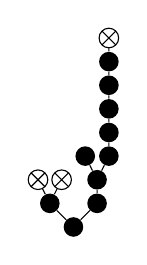
\begin{tikzpicture}[scale=.2]
\node[circle, scale=0.75, fill] (tid0) at (3,1.5){};
\node[circle, scale=0.75, fill] (tid1) at (1.5,3){};
\node[circle, scale=0.75, fill, task_scheduled] (tid3) at (0.75,4.5){};
\node[circle, scale=0.75, fill, task_scheduled] (tid4) at (2.25,4.5){};
\draw[](tid1) -- (tid3);
\draw[](tid1) -- (tid4);
\node[circle, scale=0.75, fill] (tid2) at (4.5,3){};
\node[circle, scale=0.75, fill] (tid5) at (4.5,4.5){};
\node[circle, scale=0.75, fill] (tid6) at (3.75,6){};
\node[circle, scale=0.75, fill] (tid7) at (5.25,6){};
\node[circle, scale=0.75, fill] (tid8) at (5.25,7.5){};
\node[circle, scale=0.75, fill] (tid9) at (5.25,9){};
\node[circle, scale=0.75, fill] (tid10) at (5.25,10.5){};
\node[circle, scale=0.75, fill] (tid11) at (5.25,12){};
\node[circle, scale=0.75, fill, task_scheduled] (tid12) at (5.25,13.5){};
\draw[](tid11) -- (tid12);
\draw[](tid10) -- (tid11);
\draw[](tid9) -- (tid10);
\draw[](tid8) -- (tid9);
\draw[](tid7) -- (tid8);
\draw[](tid5) -- (tid6);
\draw[](tid5) -- (tid7);
\draw[](tid2) -- (tid5);
\draw[](tid0) -- (tid1);
\draw[](tid0) -- (tid2);
\end{tikzpicture}
\nodepart{two}
\footnotesize{9.06594}
\nodepart{three}
\footnotesize{$33\:67$}
};
 & 
\node[draw=black, rectangle split,  rectangle split parts=3] (sn0x83858e8){
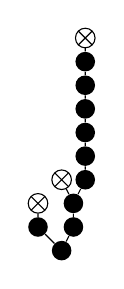
\begin{tikzpicture}[scale=.2]
\node[circle, scale=0.75, fill] (tid0) at (2.25,1.5){};
\node[circle, scale=0.75, fill] (tid1) at (0.75,3){};
\node[circle, scale=0.75, fill, task_scheduled] (tid3) at (0.75,4.5){};
\draw[](tid1) -- (tid3);
\node[circle, scale=0.75, fill] (tid2) at (3,3){};
\node[circle, scale=0.75, fill] (tid4) at (3,4.5){};
\node[circle, scale=0.75, fill, task_scheduled] (tid5) at (2.25,6){};
\node[circle, scale=0.75, fill] (tid6) at (3.75,6){};
\node[circle, scale=0.75, fill] (tid7) at (3.75,7.5){};
\node[circle, scale=0.75, fill] (tid8) at (3.75,9){};
\node[circle, scale=0.75, fill] (tid9) at (3.75,10.5){};
\node[circle, scale=0.75, fill] (tid10) at (3.75,12){};
\node[circle, scale=0.75, fill] (tid11) at (3.75,13.5){};
\node[circle, scale=0.75, fill, task_scheduled] (tid12) at (3.75,15){};
\draw[](tid11) -- (tid12);
\draw[](tid10) -- (tid11);
\draw[](tid9) -- (tid10);
\draw[](tid8) -- (tid9);
\draw[](tid7) -- (tid8);
\draw[](tid6) -- (tid7);
\draw[](tid4) -- (tid5);
\draw[](tid4) -- (tid6);
\draw[](tid2) -- (tid4);
\draw[](tid0) -- (tid1);
\draw[](tid0) -- (tid2);
\end{tikzpicture}
\nodepart{two}
\footnotesize{10.0202}
\nodepart{three}
\footnotesize{$33\:33\:33$}
};
 & 
\\
};
\end{scope}
\begin{scope}[yshift=\leveltopIII cm]
\matrix (line3)[column sep=0.5cm] {
\node[draw=black, rectangle split,  rectangle split parts=3] (sn0x8387830){
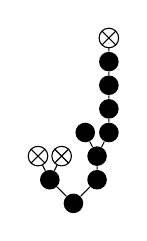
\begin{tikzpicture}[scale=.2]
\node[circle, scale=0.75, fill] (tid0) at (3,1.5){};
\node[circle, scale=0.75, fill] (tid1) at (1.5,3){};
\node[circle, scale=0.75, fill, task_scheduled] (tid3) at (0.75,4.5){};
\node[circle, scale=0.75, fill, task_scheduled] (tid4) at (2.25,4.5){};
\draw[](tid1) -- (tid3);
\draw[](tid1) -- (tid4);
\node[circle, scale=0.75, fill] (tid2) at (4.5,3){};
\node[circle, scale=0.75, fill] (tid5) at (4.5,4.5){};
\node[circle, scale=0.75, fill] (tid6) at (3.75,6){};
\node[circle, scale=0.75, fill] (tid7) at (5.25,6){};
\node[circle, scale=0.75, fill] (tid8) at (5.25,7.5){};
\node[circle, scale=0.75, fill] (tid9) at (5.25,9){};
\node[circle, scale=0.75, fill] (tid10) at (5.25,10.5){};
\node[circle, scale=0.75, fill, task_scheduled] (tid11) at (5.25,12){};
\draw[](tid10) -- (tid11);
\draw[](tid9) -- (tid10);
\draw[](tid8) -- (tid9);
\draw[](tid7) -- (tid8);
\draw[](tid5) -- (tid6);
\draw[](tid5) -- (tid7);
\draw[](tid2) -- (tid5);
\draw[](tid0) -- (tid1);
\draw[](tid0) -- (tid2);
\end{tikzpicture}
\nodepart{two}
\footnotesize{8.12123}
\nodepart{three}
\footnotesize{$33\:67$}
};
 & 
\node[draw=black, rectangle split,  rectangle split parts=3] (sn0x83857c8){
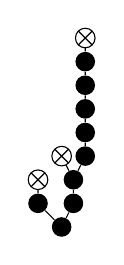
\begin{tikzpicture}[scale=.2]
\node[circle, scale=0.75, fill] (tid0) at (2.25,1.5){};
\node[circle, scale=0.75, fill] (tid1) at (0.75,3){};
\node[circle, scale=0.75, fill, task_scheduled] (tid3) at (0.75,4.5){};
\draw[](tid1) -- (tid3);
\node[circle, scale=0.75, fill] (tid2) at (3,3){};
\node[circle, scale=0.75, fill] (tid4) at (3,4.5){};
\node[circle, scale=0.75, fill, task_scheduled] (tid5) at (2.25,6){};
\node[circle, scale=0.75, fill] (tid6) at (3.75,6){};
\node[circle, scale=0.75, fill] (tid7) at (3.75,7.5){};
\node[circle, scale=0.75, fill] (tid8) at (3.75,9){};
\node[circle, scale=0.75, fill] (tid9) at (3.75,10.5){};
\node[circle, scale=0.75, fill] (tid10) at (3.75,12){};
\node[circle, scale=0.75, fill, task_scheduled] (tid11) at (3.75,13.5){};
\draw[](tid10) -- (tid11);
\draw[](tid9) -- (tid10);
\draw[](tid8) -- (tid9);
\draw[](tid7) -- (tid8);
\draw[](tid6) -- (tid7);
\draw[](tid4) -- (tid5);
\draw[](tid4) -- (tid6);
\draw[](tid2) -- (tid4);
\draw[](tid0) -- (tid1);
\draw[](tid0) -- (tid2);
\end{tikzpicture}
\nodepart{two}
\footnotesize{9.03829}
\nodepart{three}
\footnotesize{$33\:33\:33$}
};
 & 
\node[draw=black, rectangle split,  rectangle split parts=3] (sn0x83843c8){
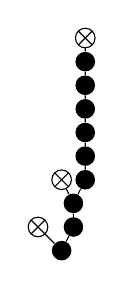
\begin{tikzpicture}[scale=.2]
\node[circle, scale=0.75, fill] (tid0) at (2.25,1.5){};
\node[circle, scale=0.75, fill, task_scheduled] (tid1) at (0.75,3){};
\node[circle, scale=0.75, fill] (tid2) at (3,3){};
\node[circle, scale=0.75, fill] (tid3) at (3,4.5){};
\node[circle, scale=0.75, fill, task_scheduled] (tid4) at (2.25,6){};
\node[circle, scale=0.75, fill] (tid5) at (3.75,6){};
\node[circle, scale=0.75, fill] (tid6) at (3.75,7.5){};
\node[circle, scale=0.75, fill] (tid7) at (3.75,9){};
\node[circle, scale=0.75, fill] (tid8) at (3.75,10.5){};
\node[circle, scale=0.75, fill] (tid9) at (3.75,12){};
\node[circle, scale=0.75, fill] (tid10) at (3.75,13.5){};
\node[circle, scale=0.75, fill, task_scheduled] (tid11) at (3.75,15){};
\draw[](tid10) -- (tid11);
\draw[](tid9) -- (tid10);
\draw[](tid8) -- (tid9);
\draw[](tid7) -- (tid8);
\draw[](tid6) -- (tid7);
\draw[](tid5) -- (tid6);
\draw[](tid3) -- (tid4);
\draw[](tid3) -- (tid5);
\draw[](tid2) -- (tid3);
\draw[](tid0) -- (tid1);
\draw[](tid0) -- (tid2);
\end{tikzpicture}
\nodepart{two}
\footnotesize{10.0097}
\nodepart{three}
\footnotesize{$33\:33\:33$}
};
 & 
\node[draw=black, rectangle split,  rectangle split parts=3] (sn0x8384e80){
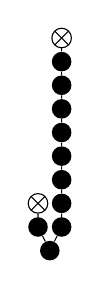
\begin{tikzpicture}[scale=.2]
\node[circle, scale=0.75, fill] (tid0) at (1.5,1.5){};
\node[circle, scale=0.75, fill] (tid1) at (0.75,3){};
\node[circle, scale=0.75, fill, task_scheduled] (tid3) at (0.75,4.5){};
\draw[](tid1) -- (tid3);
\node[circle, scale=0.75, fill] (tid2) at (2.25,3){};
\node[circle, scale=0.75, fill] (tid4) at (2.25,4.5){};
\node[circle, scale=0.75, fill] (tid5) at (2.25,6){};
\node[circle, scale=0.75, fill] (tid6) at (2.25,7.5){};
\node[circle, scale=0.75, fill] (tid7) at (2.25,9){};
\node[circle, scale=0.75, fill] (tid8) at (2.25,10.5){};
\node[circle, scale=0.75, fill] (tid9) at (2.25,12){};
\node[circle, scale=0.75, fill] (tid10) at (2.25,13.5){};
\node[circle, scale=0.75, fill, task_scheduled] (tid11) at (2.25,15){};
\draw[](tid10) -- (tid11);
\draw[](tid9) -- (tid10);
\draw[](tid8) -- (tid9);
\draw[](tid7) -- (tid8);
\draw[](tid6) -- (tid7);
\draw[](tid5) -- (tid6);
\draw[](tid4) -- (tid5);
\draw[](tid2) -- (tid4);
\draw[](tid0) -- (tid1);
\draw[](tid0) -- (tid2);
\end{tikzpicture}
\nodepart{two}
\footnotesize{10.0127}
\nodepart{three}
\footnotesize{$50\:50$}
};
 & 
\\
};
\end{scope}
\draw (sn0x8387a30.south) -- (sn0x83858e8.north);
\draw (sn0x8387a30.south) -- (sn0x8387918.north);
\draw (sn0x8387918.south) -- (sn0x83857c8.north);
\draw (sn0x8387918.south) -- (sn0x8387830.north);
\draw (sn0x83858e8.south) -- (sn0x83843c8.north);
\draw (sn0x83858e8.south) -- (sn0x8384e80.north);
\draw (sn0x83858e8.south) -- (sn0x83857c8.north);
\end{tikzpicture}
%%% Local Variables:
%%% TeX-master: "thesis/thesis.tex"
%%% End: 
      
      \end{column}
    \end{columns}
  \end{counterexampleblock}
\end{frame}

\subsection{Only highest or lowest leaves}

\begin{frame}
  \frametitle{Only highest and lowest leaves}
  \begin{motivationblock}
    All optimal schedules seen so far scheduled only highest and lowest possible leaves.
  \end{motivationblock}
  \begin{strategyblock}
    Restrict to snapshots where only highest and lowest leaves are scheduled.
  \end{strategyblock}
  \begin{counterexampleblock}
    \begin{columns}
      \begin{column}{.5\textwidth}
        \begin{center}
          \renewcommand{\leveltopI}{-16cm + \leveltop}
\renewcommand{\leveltopII}{-16cm + \leveltopI}
\renewcommand{\leveltopIII}{-16cm + \leveltopII}
\renewcommand{\leveltopIIII}{-16cm + \leveltopIII}
\renewcommand{\leveltopIIIII}{-16cm + \leveltopIIII}
\renewcommand{\leveltopIIIIII}{-16cm + \leveltopIIIII}
\renewcommand{\leveltopIIIIIII}{-16cm + \leveltopIIIIII}
\renewcommand{\leveltopIIIIIIII}{-16cm + \leveltopIIIIIII}
\renewcommand{\leveltopIIIIIIIII}{-16cm + \leveltopIIIIIIII}
\renewcommand{\leveltopIIIIIIIIII}{-16cm + \leveltopIIIIIIIII}
\renewcommand{\leveltopIIIIIIIIIII}{-16cm + \leveltopIIIIIIIIII}
\renewcommand{\leveltopIIIIIIIIIIII}{-16cm + \leveltopIIIIIIIIIII}
\renewcommand{\leveltopIIIIIIIIIIIII}{-16cm + \leveltopIIIIIIIIIIII}
\begin{tikzpicture}[scale=.2, anchor=south]
\begin{scope}[yshift=\leveltopI cm]
\matrix (line1)[column sep=0.5cm] {
\node[draw=black, rectangle split,  rectangle split parts=2] (sn0x9b5bc80){
\begin{tikzpicture}[scale=.2]
\node[circle, scale=0.75, fill] (tid0) at (3.75,1.5){};
\node[circle, scale=0.75, fill] (tid1) at (0.75,3){};
\node[circle, scale=0.75, fill] (tid2) at (2.25,3){};
\node[circle, scale=0.75, fill] (tid4) at (2.25,4.5){};
\node[circle, scale=0.75, fill] (tid6) at (2.25,6){};
\draw[](tid4) -- (tid6);
\draw[](tid2) -- (tid4);
\node[circle, scale=0.75, fill] (tid3) at (5.25,3){};
\node[circle, scale=0.75, fill] (tid5) at (5.25,4.5){};
\node[circle, scale=0.75, fill] (tid7) at (5.25,6){};
\node[circle, scale=0.75, fill, task_scheduled] (tid8) at (3.75,7.5){};
\node[circle, scale=0.75, fill] (tid9) at (6,7.5){};
\node[circle, scale=0.75, fill] (tid10) at (6,9){};
\node[circle, scale=0.75, fill, task_scheduled] (tid11) at (5.25,10.5){};
\node[circle, scale=0.75, fill, task_scheduled] (tid12) at (6.75,10.5){};
\draw[](tid10) -- (tid11);
\draw[](tid10) -- (tid12);
\draw[](tid9) -- (tid10);
\draw[](tid7) -- (tid8);
\draw[](tid7) -- (tid9);
\draw[](tid5) -- (tid7);
\draw[](tid3) -- (tid5);
\draw[](tid0) -- (tid1);
\draw[](tid0) -- (tid2);
\draw[](tid0) -- (tid3);
\end{tikzpicture}
\nodepart{two}
\footnotesize{7.79154}
};
\\
};
\end{scope}
\end{tikzpicture}
%%% Local Variables:
%%% TeX-master: "thesis/thesis.tex"
%%% End: 

        \end{center}      
      \end{column}
      \begin{column}{.5\textwidth}
        \begin{center}
          \input{00023457791010_opt}
        \end{center}      
      \end{column}
    \end{columns}
  \end{counterexampleblock}
\end{frame}

\subsection{As few free paths as possible}

\begin{frame}
  \frametitle{As few free paths as possible}
  \begin{motivationblock}
    \begin{itemize}
    \item A path from the root to a leaf is \emph{free}, if \emph{no} task on the path has a scheduled predecessor
    \item Some non-HLF examples are optimally scheduled by a strategy that minimizes the number of free paths
    \item We tried it as a heuristic for can-optimal HLF
    \end{itemize}
  \end{motivationblock}
  \todo{Kurzes Bild}
\end{frame}

\begin{frame}
  \frametitle{As few free paths as possible}
  \begin{strategyblock}
    When scheduler has a choice, minimize the number of free paths.
  \end{strategyblock}
  \todo{Bild.}
\end{frame}

\subsection{Subtree with fewer topmost tasks}

\begin{frame}
  \frametitle{Subtree with fewer topmost tasks}
  \begin{motivationblock}
    In many cases, a topmost task being the single requirement for its direct successor has to be scheduled
  \end{motivationblock}
  \begin{definition}[Topmost-maximal subtree for a leaf]
    Let $t$ be a leaf and let $p=(t, t_1, t_2, t_3, \dots, r)$ be the path from $t$ to the root $r$.

    The \emph{topmost-maximal subtree} for $t$ is the subtree rooted at the \emph{lowest} task $t^*$ within $p$ different from $t$ that does \emph{not} contain more topmost tasks than the subtree rooted at the direct successor of $t$. 
  \end{definition}
\end{frame}


\definecolor{topmosttask}{rgb}{0.8,0.3,0}
\definecolor{currenttask}{rgb}{0.3,.5,0.2}
\definecolor{donetask}{HTML}{EFCC3C}

\begin{frame}
  \frametitle{Subtree with fewer topmost tasks}
  \begin{columns}
    \begin{column}{.3\textwidth}
      \begin{exampleblock}{Example intree}
        \begin{center}
          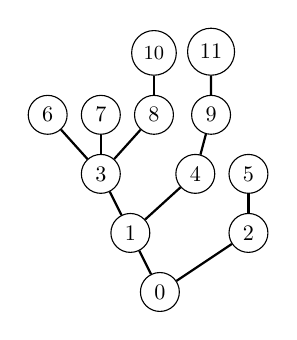
\begin{tikzpicture}[scale=.5, anchor=south]
            \node[circle, scale=0.8, draw] (tid0) at (3,1.5){0};
            \node[circle, scale=0.8, draw, onslide=<5>{fill=currenttask}] (tid1) at (2.25,3){1};
            \node[circle, scale=0.8, draw, onslide=<4>{fill=currenttask}, onslide=<5->{fill=donetask}] (tid2) at (1.5,4.5){3};
            \node[circle, scale=0.8, draw, onslide=<4->{fill=donetask}] (tid7) at (0.15,6){6};
            \node[circle, scale=0.8, draw, onslide=<4->{fill=donetask}] (tid10) at (1.5,6){7};
            \draw[ thick](tid2) -- (tid7);
            \draw[ thick](tid2) -- (tid10);
            \node[circle, scale=0.8, draw, onslide=<5>{fill=donetask}] (tid3) at (3.9,4.5){4};
            \node[circle, scale=0.8, draw, onslide=<3>{fill=currenttask}, onslide=<4->{fill=donetask}] (tid5) at (2.85,6){8};
            \node[circle, scale=0.8, draw, onslide=<2>{fill=currenttask}, onslide=<3-5>{fill=topmosttask}, onslide=<6>{fill=donetask}] (tid6) at (2.85,7.5){\small 10};
            \draw[ thick](tid5) -- (tid6);
            \draw[ thick](tid2) -- (tid5);
            \draw[ thick](tid1) -- (tid2);
            \draw[ thick](tid1) -- (tid3);
            \node[circle, scale=0.8, draw] (tid4) at (5.25,3){2};
            \node[circle, scale=0.8, draw, onslide=<5>{fill=donetask}] (tid9) at (4.3,6){9};
            \draw[ thick](tid3) -- (tid9);
            \node[circle, scale=0.8, draw, onslide=<5>{fill=topmosttask}] (tid11) at (4.3,7.5){11};
            \draw[ thick](tid11) -- (tid9);
            \node[circle, scale=0.8, draw] (tid8) at (5.25,4.5){5};
            \draw[ thick](tid4) -- (tid8);
            \draw[ thick](tid0) -- (tid1);
            \draw[ thick](tid0) -- (tid4);
          \end{tikzpicture}
        \end{center}
      \end{exampleblock}
    \end{column}
    \begin{column}{.7\textwidth}
      Topmost-maximal subtree for task 10:
      \begin{itemize}
      \item<2-> The subtree rooted at 10 (called $I_{10}$) contains only the topmost task 10 (omitted). %It is omitted because we want to find the lowest task along the path that is different from 10.
      \item<3-> Subtree $I_8$ contains only topmost task 10 (reference).
      \item<4-> Subtree $I_3$ still contains only 10 as the topmost task (it introduces only new \emph{leaves}, namely 6 and 7).
      \item<5-> Subtree $I_1$ contains 10 \emph{and} 11 as topmost tasks.
      \item<6-> Subtree $I_3$ is the topmost maximal subtree for task 10.
      \end{itemize}
    \end{column}
  \end{columns}
\end{frame}


\begin{frame}
  \frametitle{Subtree with fewer topmost tasks}
  \begin{strategyblock}
    Prefer tasks whose topmost-maximal subtree has fewer topmost tasks.
  \end{strategyblock}
  \begin{counterexampleblock}
    \todo{Bild!}
  \end{counterexampleblock}
\end{frame}

\subsection{Subtree with fewer leaves}

\begin{frame}
  \frametitle{Subtree with fewer leaves}
  \begin{motivationblock}
    Maybe we were wrong and should have focussed on \emph{ready}, and not on \emph{topmost} tasks.
  \end{motivationblock}
  \begin{definition}[Leaf-maximal subtree for a leaf]
    Let $t$ be a leaf and let $p=(t, t_1, t_2, t_3, \dots, r)$ be the path from $t$ to the root $r$.

    The \emph{leaf-maximal subtree} for $t$ is the subtree rooted at the \emph{lowest} task $t^*$ within $p$ different from $t$ that does \emph{not} contain more leaves than the subtree rooted at the direct successor of $t$. 
  \end{definition}
  \emph{Remark:} Preferring subtrees with more does not work.
\end{frame}

\begin{frame}
  \frametitle{Subtree with fewer leaves}
  \begin{strategyblock}
    Prefer tasks whose leaf-maximal subtree has fewer topmost tasks.
  \end{strategyblock}
  \begin{counterexampleblock}
    \todo{Bild.}
  \end{counterexampleblock}
\end{frame}

\subsection{Filling up subtrees}

\begin{frame}
  \frametitle{Filling up subtrees}
  \begin{motivationblock}
    Subtrees seem to be filled up one after another.
  \end{motivationblock}
  \begin{counterexampleblock}
    \begin{center}
      \input{00023355666_opt}
    \end{center}
  \end{counterexampleblock}
\end{frame}

\subsection{Maximizing $T_3$, minimizing $T_1$}

\begin{frame}
  \frametitle{Maximizing 3-processor time, minimizing 1-processor
    time}
  \begin{block}{Optimal schedules do \emph{not} necessarily \dots}
    \begin{itemize}
    \item \dots maximize the expected time span $T_3$ where 3 processors are busy
    \item \dots minimize the expected time span $T_1$ where only 1 processor can work
    \end{itemize}
  \end{block}
  \begin{columns}
    \begin{column}{.3\textwidth}
      \begin{center}
        \input{00112333_t1min}
        $T_1=2.98$
      \end{center}
    \end{column}
    \begin{column}{.3\textwidth}
      \begin{center}
        \input{00112333_t3max} 
        $T_3=2.36$
      \end{center}
    \end{column}
    \begin{column}{.4\textwidth}
      \begin{center}
        \renewcommand{\leveltopI}{-13cm + \leveltop}
\renewcommand{\leveltopII}{-13cm + \leveltopI}
\renewcommand{\leveltopIII}{-13cm + \leveltopII}
\renewcommand{\leveltopIIII}{-13cm + \leveltopIII}
\renewcommand{\leveltopIIIII}{-13cm + \leveltopIIII}
\renewcommand{\leveltopIIIIII}{-13cm + \leveltopIIIII}
\renewcommand{\leveltopIIIIIII}{-13cm + \leveltopIIIIII}
\renewcommand{\leveltopIIIIIIII}{-13cm + \leveltopIIIIIII}
\renewcommand{\leveltopIIIIIIIII}{-13cm + \leveltopIIIIIIII}
\begin{tikzpicture}[scale=.2, anchor=south]
\begin{scope}[yshift=\leveltopI cm]
\matrix (line1)[column sep=1cm] {
\node[draw=black, rectangle split,  rectangle split parts=2] (sn0x957bcd0){
\begin{tikzpicture}[scale=.2]
\node[circle, scale=0.75, fill] (tid0) at (3.75,1.5){};
\node[circle, scale=0.75, fill] (tid1) at (3,3){};
\node[circle, scale=0.75, fill] (tid3) at (0.75,4.5){};
\node[circle, scale=0.75, fill] (tid4) at (3.75,4.5){};
\node[circle, scale=0.75, fill, task_scheduled] (tid6) at (2.25,6){};
\node[circle, scale=0.75, fill, task_scheduled] (tid7) at (3.75,6){};
\node[circle, scale=0.75, fill, task_scheduled] (tid8) at (5.25,6){};
\draw[](tid4) -- (tid6);
\draw[](tid4) -- (tid7);
\draw[](tid4) -- (tid8);
\draw[](tid1) -- (tid3);
\draw[](tid1) -- (tid4);
\node[circle, scale=0.75, fill] (tid2) at (6.75,3){};
\node[circle, scale=0.75, fill] (tid5) at (6.75,4.5){};
\draw[](tid2) -- (tid5);
\draw[](tid0) -- (tid1);
\draw[](tid0) -- (tid2);
\end{tikzpicture}
\nodepart{two}
\footnotesize{5.3287}
};
\\
};
\end{scope}
\end{tikzpicture}
%%% Local Variables:
%%% TeX-master: "thesis/thesis.tex"
%%% End: 
 
        $T_3=2.33, T_1=2.99$
      \end{center}
    \end{column}
  \end{columns}
\end{frame}

\end{document}

%%% Local Variables: 
%%% mode: latex
%%% TeX-master: t
%%% End: 
